\documentclass[12pt]{article}
\usepackage[utf8]{inputenc}
\usepackage{Preambles/preamble}
\usepackage{biblatex}
\usepackage{pgfplots}
\usepackage{tikz}
\usepackage{float}
\usepackage{graphicx}

\addbibresource{References.bib}
%~~~~~~~~~~~~~~~~~~~~~~~~~~~~~~~~~~~~~~~~~~~~~~~~~~~~~~~~~~~~~~~~~~~~~~~~~~~~~~~~~~~~~~~~~~~~~~%
%%%%%%%%%%%%%%%%%%%%%%%%%%%%%%%%%%%%%%%%%%%%%%%%%%%%%%%%%%%%%%%%%%%%%%%%%%%%%%%%%%%%%%%%%%%%%%%%
%                                                                                              % 
%             Template produced by Fergus Babb of the University of Nottingham, 2024           %
%                                                                                              %  
%%%%%%%%%%%%%%%%%%%%%%%%%%%%%%%%%%%%%%%%%%%%%%%%%%%%%%%%%%%%%%%%%%%%%%%%%%%%%%%%%%%%%%%%%%%%%%%%
%~~~~~~~~~~~~~~~~~~~~~~~~~~~~~~~~~~~~~~~~~~~~~~~~~~~~~~~~~~~~~~~~~~~~~~~~~~~~~~~~~~~~~~~~~~~~~~%

\begin{document}

%%%%%%%%%%%%%%%%%%%%%%%%%%%%%%%%%%%%%%%%%%%%%%%%%%%%%%%%%%%%%%%%%%%%%%%%%%%%%%%%%%%%%%%%%%%%%%%%
\title{Ion and neutral uniformity in SF6 plasmas with tailored voltage waveforms}
%This isn't supposed to be for level of authorship, alphabetical is fine
\firstauthor{Matthew Robertson}

\firstemail{matthew.robertson@gaxau.com}

\submitdate{\today}
\maketitle

\addtocounter{page}{-1}
\pagenumbering{roman}
\thispagestyle{empty}
%%%%%%%%%%%%%%%%%%%%%%%%%%%%%%%%%%%%%%%%%%%%%%%%%%%%%%%%%%%%%%%%%%%%%%%%%%%%%%%%%%%%%%%%%%%%%%%%


%~~~~~~~~~~~~~~~~~~~~~~~~~~~~~~~~~~~~~~~~~~~~~~~~~~~~~~~~~~~~~~~~~~~~~~~~~~~~~~~~~~~~~~~~~~~~~~~

\newpage
\doublespacing
\tableofcontents
\singlespacing

%~~~~~~~~~~~~~~~~~~~~~~~~~~~~~~~~~~~~~~~~~~~~~~~~~~~~~~~~~~~~~~~~~~~~~~~~~~~~~~~~~~~~~~~~~~~~~~~
%Sections before Main Content of report






%~~~~~~~~~~~~~~~~~~~~~~~~~~~~~~~~~~~~~~~~~~~~~~~~~~~~~~~~~~~~~~~~~~~~~~~~~~~~~~~~~~~~~~~~~~~~~~~
%Main Content sections start

\newpage
\pagenumbering{arabic}
\section*{Main Content}%So pdf viewers dont have everything as a subsection of preamble
\addcontentsline{toc}{part}{Main Content}

\section{Abstract} \label{Sec: Abstract}

Semiconductor manufacturers use plasma to etch silicon wafers for extreme precision, however, issues lie in ensuring plasma uniformity along the edges of the wafer potentially meaning more defects and manufacturing error. Work presented aims to investigate how modifying the RF bias waveform affects positive ion and neutral uniformity for fluorine from SF6 dissociation using simulations ran in the HPEM (Hybrid Plasma Equipment Model). Specifically we make use of the 'peak and valley' and 'sawtooth' tailored waveforms as presented in \cite{Doyle2020}



\section{Introduction}\label{Sec: Introduction}

The uniformity of ion and neutral flux across the wafer surface is a critical factor in semiconductor plasma processing. Non-uniform plasma ion fluxes can lead to uneven etching, particularly near wafer edges, introducing defects and reducing overall device yield. As the demand for semiconductor devices continues to increase, the industry has responded with larger wafer sizes, increasing from the standard 150mm wafer to 200mm, with plans to expand further. Maintaining a uniform ion etch across larger wafers requires reconsidering long applied etching techniques and the development of new plasma control techniques.

One attractive approach to improving flux uniformity involves modifying the shape of the applied RF bias voltage waveform. Unlike mechanical modifications to the reactor geometry or hardware changes to the RF system, waveform tailoring is a low-cost and non-invasive solution. It requires no physical alteration of the reactor, avoids extended downtime, and can be implemented through relatively straightforward changes in the driving electronics. This makes it a practical strategy for rapid process optimisation in both research and industrial environments.

In this work, we investigate the effect of tailored RF waveforms specifically, 'peak and valley' and 'sawtooth' forms on the uniformity of fluorine ion and neutral fluxes on a dielectric wafer produced from SF$_6$ plasma in a Gaseous Electronic Cell (GEC) geometry. Simulations are performed using the Hybrid Plasma Equipment Model (HPEM), a modular and widely validated plasma simulation framework.

% Aims included within Introduction - What we want to achieve.


%~~~~~~~~~~~~~~~~~~~~~~~~~~~~~~~~~~~~~~~~~~~~~~~~~~~~~~~~~~~~~~~~~~~~~~~~~~~~~~~~~~~~~~~~~~~~~~~
\newpage
\section{Modelling}\label{Sec: Modelling}

\subsection{HPEM}

The HPEM (Hybrid Plasma Equipment Model) is a sophisticated and modular model for plasmas. Originally created by Mark J. Kushner \cite{Kushner2009} and has been maintained and expanded upon by various academics all across the globe.

A high-level overview of how the HPEM works can be seen in \ref{fig:HPEM}.

\begin{figure}[H]
    \centering
    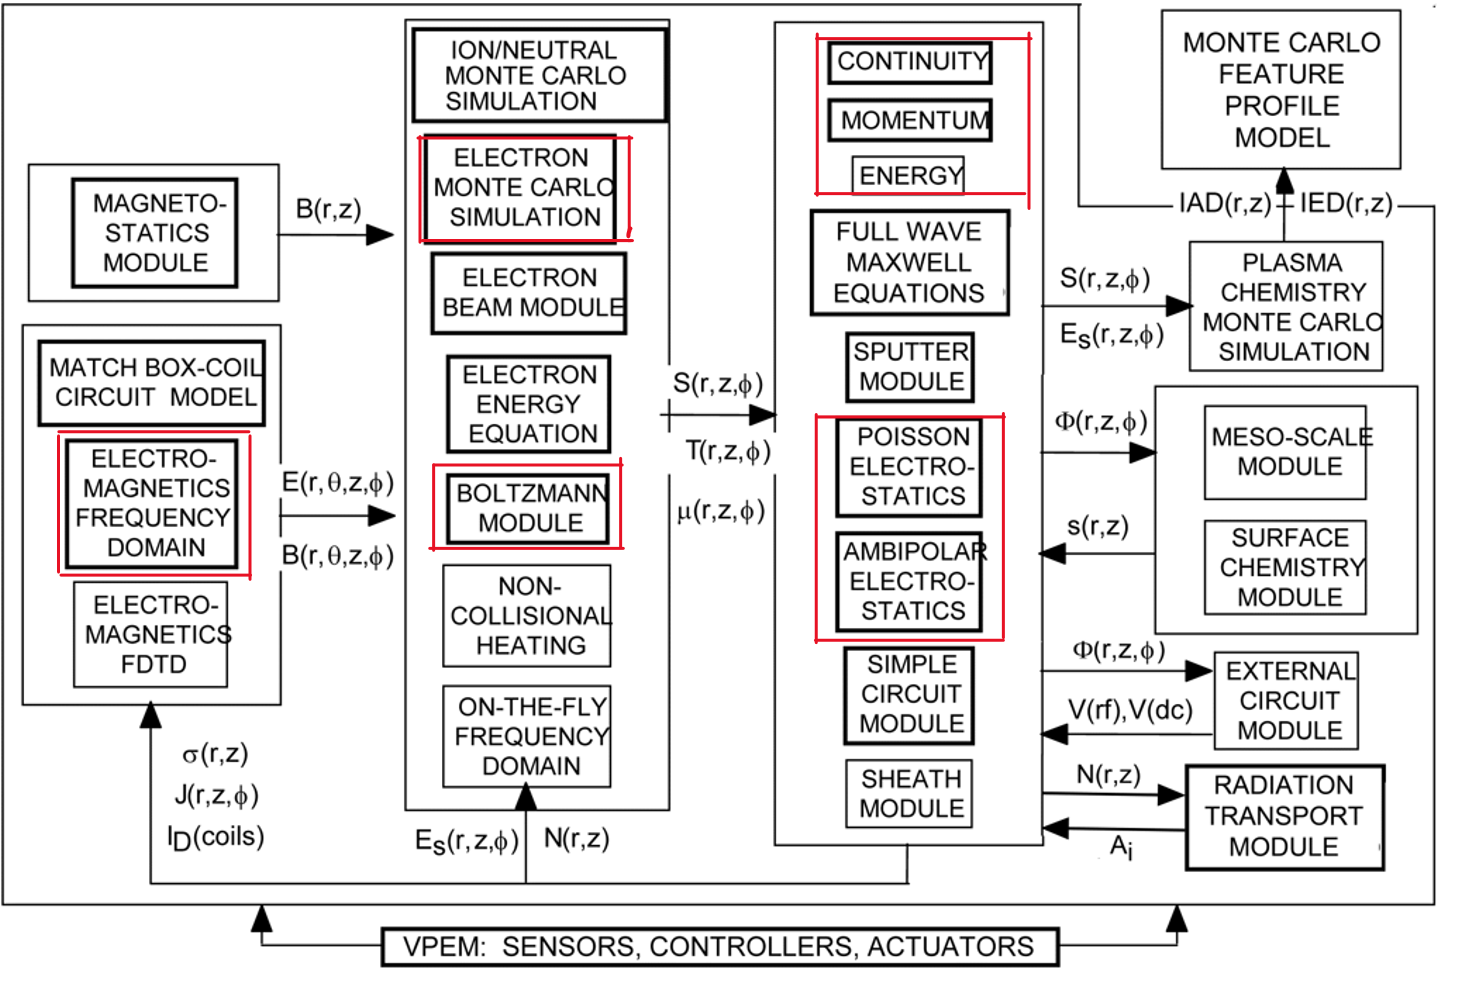
\includegraphics[width=\linewidth]{Figures/HPEM.png}
    \caption{HPEM Workflow}
    \label{fig:HPEM}
\end{figure}

The HPEM workflow proceeds in an iterative manner, integrating multiple physical models \cite{Smith2024,Doyle2024}:

\begin{enumerate}
    \item{\textbf{Semi-implicit Poisson Solver \& Electromagnetics Frequency Domain (EMFD)}} \\
    Solves for charge density "rho" at the vertices of each cell based on the total number of charged species. From that, we obtain the electric potential at the same location via a semi-implicit Poisson solution, considering electron diffusion. The electric field at each location is then obtained via a 3-molecule half-step spatial gradient between adjacent cell vertices.

    \item{\textbf{Electron Monte Carlo Simulation (EMCS)}} \\
    Tracks electron trajectories under the calculated electric field. Used when electron energy distributions are non-Maxwellian, making the Boltzmann approximation invalid. Outputs spatially resolved electron densities, energies, and energy distribution functions.

    \item{\textbf{Boltzmann Module}} \\
    Applied for ions and other species with near-Maxwellian distributions. Calculates transport coefficients, mobilities, and diffusion rates for heavy charged species.

    \item{\textbf{Plasma Chemistry Solver}} \\
    Uses the species densities and energies to solve coupled continuity, momentum, and energy conservation equations. Simultaneously solves Poisson’s equation for electrostatics and the ambipolar electrostatic equations for ion-electron coupling.

    \item{Feedback Loop} \\
    The updated charge densities and currents ($\rho$ and $\mathbf{J}$) are fed back to the EMFD \& semi-implicit Possion solver, and the cycle repeats until convergence.
\end{enumerate}


\subsection{Geometry}

The geometry for our simulations ran in the HPEM is the GEC geometry. The Gaseous Electric Cell (GEC) geometry is a widely used and well understood geometry, that is similar but not exactly like the one used at OIPT (Oxford Instruments Plasma Technology), for our experiments the GEC geometry is satisfactory. The reactor is in the cylindrical coordinate system with a radius of 12cm and a height of 12cm. Our mesh consisted of 60 cells radially and 120 cells axially, for spatial resolutions of 0.2 [cm/cell] and 0.1 [cm/cell], respectively. The silicon wafer surface is at 3.9cm in the Z axis and ranges along 0 - 5.2cm radially. Our silicon wafer has a conductivity of $1\times10^{-16}$ S/cm and relative permittivity (6.7) of the wafer.

Baseline simulation operating conditions employed a 13.56MHz, 480V amplitude (960V peak-to-peak), sinusoidal voltage applied at the powered electrode, maintaining a capacitively coupled plasma (CCP). Tailored voltage waveforms employed 13.56MHz as their fundamental frequency, and a peak-to-peak voltage of 960~V was maintained for all waveforms. An inlet flow rate of 50sccm maintained a pressure of 10mTorr for a converged temperature of ~400K.



\begin{figure}[H]
    \centering
    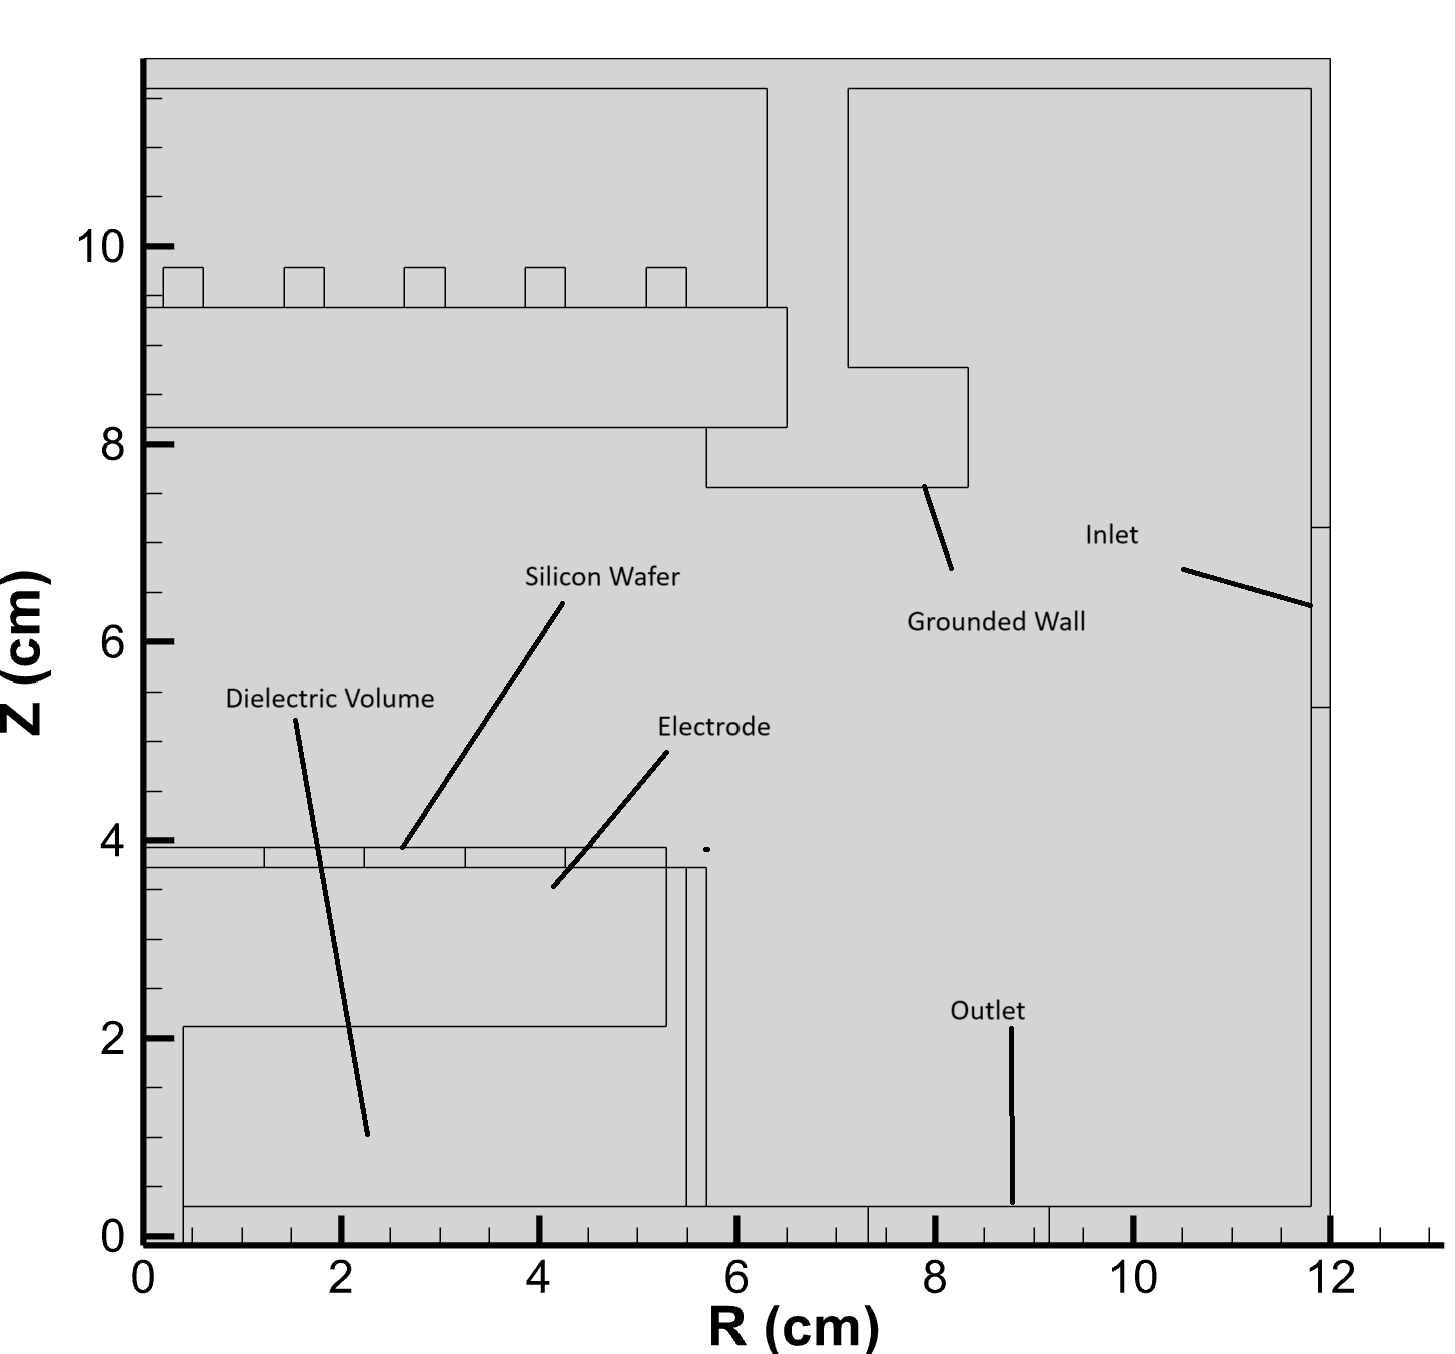
\includegraphics[width=\linewidth]{Figures/Geometry.png}
    \caption{GEC Geometry used in our simulations.}
    \label{fig:GEC_geometry}
\end{figure}

\begin{figure}[H]
    \centering
    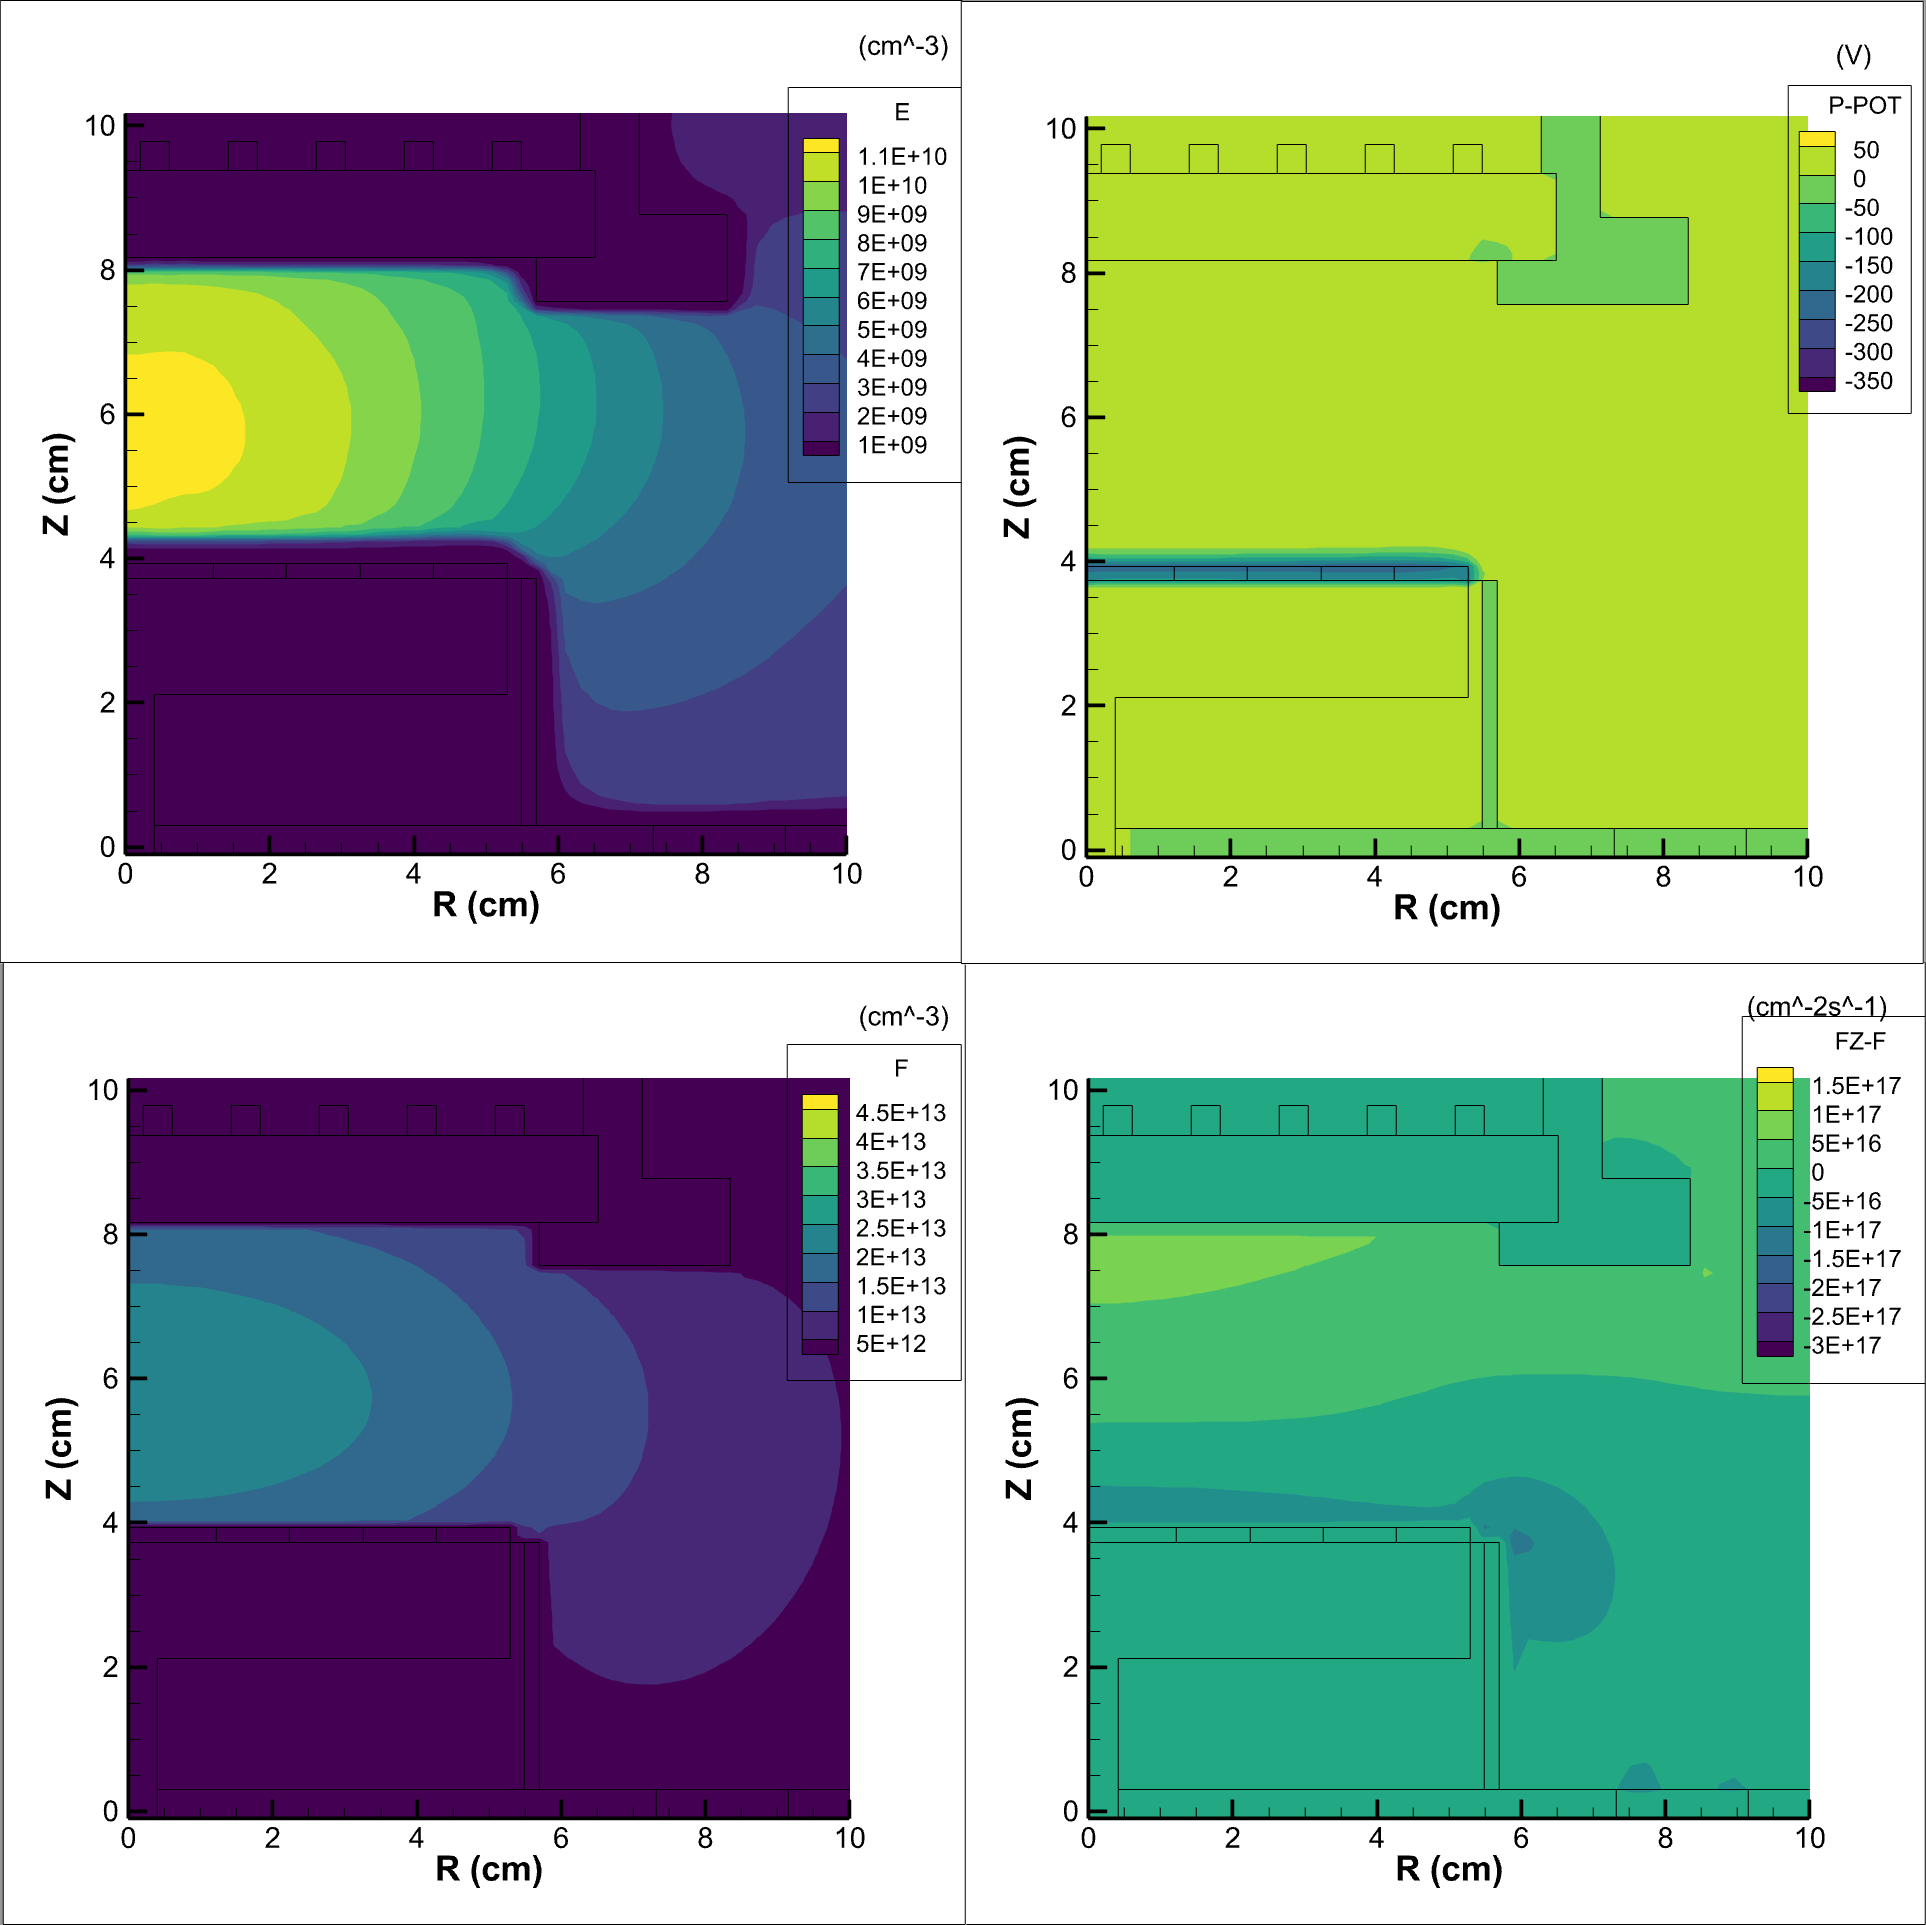
\includegraphics[width=\linewidth]{Figures/4x4 Plasma.png}
    \caption{GEC geometry with electron density, RF Bias (PPOT), fluorine density and neutral fluorine flux from our 1H13 baseline simulation.}
    \label{fig:GEC_electron_density}
\end{figure}

A baseline discharge employing a single sinusoidal 13.56MHz voltage waveform applied at the lower electrode for 50 sccm of SF6 at 10mTorr is shown in figure 3. A maximum electron density of $1.1\times10^{10} \text{cm}^{-3}$  was observed, decreasing linearly with radius, reducing approximately by a factor of 2 across the wafer surface to a value of $0.5\times10^{10} \text{cm}^{-3}$ at the edge of the wafer (R = 5cm). The bulk plasma potential reached 60V wafer accumulated a significant DC electric potential of -350V, due largely to the significant physical asymmetry of the reactor. This "DC self-bias" forms to maintain the same RF-averaged charge fluxes through both the powered and grounded surfaces, required to maintain quasineutrality. The electron density is slightly lower than would be expected for a similar argon discharge due to dissociative attachment of the SF6 gas, producing a significant bulk F- ion population (Max F- Density: $9.3\times10^{10} \text{cm}^{-3}$, Max F+ Density: $2.4\times10^{9} \text{cm}^{-3}$). Direct dissociation of $\text{SF}_x$ species is also observed, producing an abundance of atomic fluorine (max density$2.4\times10^{13} \text{cm}^{-3}$), topologically co-located with the electron density distribution and similarily decreasing linearly by a factor of ~2 with increasing radius. Neutral fluorine flux (FZ-F) is also shown, with directionality indicated by the blue (negative Z-direction) and green (positive Z-direction) regions, respectively. The flux incident upon the wafer ($3.0\times10^{17} \text{cm}^{-2}\text{s}^{-1}$) is approximately double that of the upper dielectric window ($1.5\times10^{17} \text{cm}^{-2}\text{s}^{-1}$) due to the proximity of the peak fluorine density to the wafer.

When we calculate our uniformities, we are interested in the flux hitting this surface and use the flux along this surface of ions and neutrals to calculate their respective uniformity values for each case.

We calculate the uniformity as follows: 

\begin{equation}
U = \frac{\operatorname{Max}(F) - \operatorname{Min}(F)}{2 \times \operatorname{Avg}(F)}
\label{eq:uniformity}
\end{equation}
Where $U$ represents the uniformity value for a particular configuration and $F$ is the list of fluxes along the wafer for the configuration.



\subsection{Chemistry}

The chemistry shown in \textbf{Table \ref{tab:nfx_reactions}} captures the key reaction pathways for $\text{SF}_6$ dissociation and ionisation, including both charged and neutral species. All considered species can be seen in \textbf{Table \ref{tab:species}}


\begin{table}[h!]
\centering
\caption{Species included in the reaction mechanism.}
\begin{tabular}{ll}
\hline
\textbf{} & \textbf{Species} \\
\hline
Charged Species & $e^{-}$, F$^{-}$, F$_2^{+}$ , S$^{+}$ , SF$^{+}$, SF$_2^{+}$ \\ &  SF$_3^{+}$, SF$_4^{+}$, SF$_5^{+}$, SF$_5^{-}$, SF$_6^{-}$ \\
Neutral Species & F, F$^{*}$, F$_2$ ,S ,SF ,SF$_2$, SF$_3$\\ & SF$_4$, SF$_5$, SF$_6$ \\
\hline
\label{tab:species}
\end{tabular}
\end{table}

\begin{table}[h]
\centering
\begin{tabular}{ll}
\hline
\textbf{Reaction} & \textbf{Type} \\
\hline
$e + \text{SF}_x \rightarrow \text{SF}_x + e$ & Elastic scattering \\
$e + \text{SF}_x \rightarrow \text{SF}_{x-1} + \text{F}^-$ & Dissociative electron attachment \\
$e + \text{SF}_x \rightarrow \text{SF}_{x-1} + \text{F} + e$ & Dissociative excitation \\
$e + \text{SF}_x \rightarrow \text{SF}_x^+ + e + e$ & Ionization \\
$e + \text{SF}_x \rightarrow \text{SF}_{x-n}^+ + n\text{F} + e + e$ & Dissociative ionization \\
$e + \text{SF}_x^+ \rightarrow \text{SF}_{x-1} + \text{F}$ & Dissociative recombination \\
$\text{F}^- + \text{SF}_x^+ \rightarrow \text{SF}_{x-1} + \text{F} + \text{F}$ & Dissociative ion–ion neutralization \\
\hline
\end{tabular}
\caption{Chemical reactions involving SF$_x$ molecules and electrons}
\label{tab:nfx_reactions}
\end{table}

We account for all intermediary reactions from $\text{SF}_6$ to $\text{SF}_1$:
\begin{equation}
\text{SF}_6 \rightarrow \text{SF}_5 \rightarrow \text{SF}_4 \rightarrow \text{SF}_3 \rightarrow \text{SF}_2 \rightarrow \text{SF}
\end{equation}

Each step can proceed either as a direct electron dissociation, producing a neutral fluorine, or as a dissociative attachment, producing a negative fluorine ion. $\text{SF}_6$ dissociation is often treated without consideration of the intermediate fractions, here we consider both the full dissociative tree and the formation of $\text{SF}_x$ fraction ions. This consideration leads to a wide range of neutral and ion masses within the simulation, which have unique effects on the power coupling, mass transport, and charge distribution. The simulation also takes into account atomic recombination, such as fluorine becoming molecular fluorine.  ($F \rightarrow F_2$)

Surface recombination is considered for both ions and neutrals on all material surfaces. Positive and negative ions impacting a wall recombine into neutral species with unity probability. Neutral F has an energy/temperature independent 22\% chance to recombine into molecular F2 when impacting a wall. Recombined species are returned to the gas phase via a modification of the wall-incident flux (i.e. the addition of a flux anti-normal to the wall).

\subsection{Tailored Waveforms}

Tailored waveforms consist of a superposition of multiple sinosoidal voltage waveforms and are constructed from a Fourier series to generate arbitrary Fourier series to generate arbitrary, or 
``tailored'', RF waveform inputs. They are defined mathematically as
\begin{equation}
    \phi_{\text{rf}}(t) = \sum_{k=1}^{n} \phi_k \sin(k\omega_0 t + \theta_k),
\end{equation}
where $\phi_k$ and $\theta_k$ are the amplitude and phase of the $k$th harmonic, 
respectively. This type of tailored waveform is known as the 'peak and valley' 
waveform, and has already been implemented into HPEM by Dr.\ Scott J. Doyle. 

\begin{figure}[H]
    \centering
    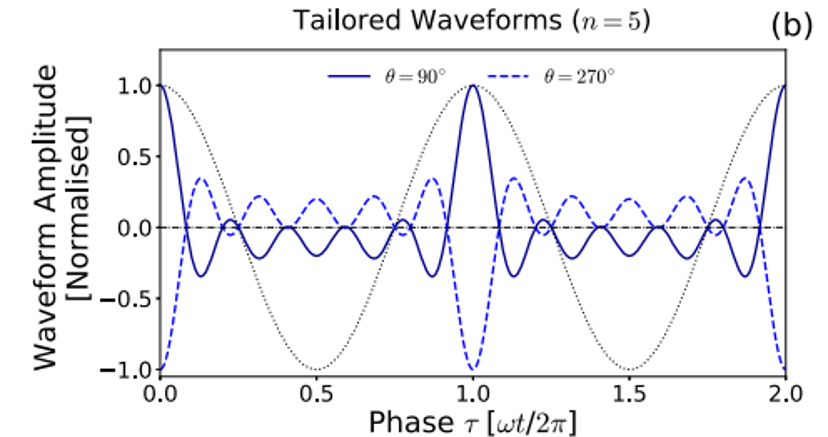
\includegraphics[width=0.75\textwidth]{Figures/TW.png} % replace with your file
    \caption{Example of the 'peak and fall' tailored waveforms constructed from $n=5$ harmonics 
    \cite{Doyle2020}.}
    \label{fig:tailored}
\end{figure}

The sawtooth tailored waveform can be defined mathematically as such:

\begin{equation}
    \phi_{\text{rf}}(t) = \sum_{k=1}^{n} \phi_k \frac{ \sin(k\omega_0 t + \theta_k)}{k},
\end{equation}

where $\phi_k$ and $\theta_k$ are the amplitude and phase of the $k$th harmonic, 
respectively. This type of tailored waveform is the sawtooth waveform 
waveform, and has also been implemented into HPEM by Dr.\ Scott J. Doyle. 

In the simulations we employ two different waveform 'shapes'; first a 'peak and valley' style waveform shown in figure 4 and generated by equation 3.3. Secondly a sawtooth style waveform, generated by equation 3.4. The peak and valley waveforms generally exhibit a two, closely located, changes in voltage, while the sawtooths generally exhibit a slow change in voltage followed by a single large change in voltage. These waveforms directly alter the plasma dynamics at the sheath, and influence the bias at the material surface. For both of these tailored waveforms we vary the phase to change the time averaged RF bias. \cite{Doyle2020,Heil2008,Lafleur2012}



%~~~~~~~~~~~~~~~~~~~~~~~~~~~~~~~~~~~~~~~~~~~~~~~~~~~~~~~~~~~~~~~~~~~~~~~~~~~~~~~~~~~~~~~~~~~~~~~
\section{Results}
\label{sec:results}

We analyse radial flux uniformity at the wafer for both neutrals and positive ions (uniformity defined in Eq.~\ref{eq:uniformity}), we also look at the measured RF bias for \emph{peak-and-fall} (PF) and \emph{sawtooth} waveforms.

\subsection{Uniformity of neutrals and positive ions}
Figures~\ref{fig:neut_u} and \ref{fig:ion_u} plot uniformity $U$ versus average flux for neutrals and positive ions, respectively, with baseline harmonic cases (1H13, 2H27, 3H40, 4H54) highlighted for reference.

All tailored voltage cases use the same pressures and flow rates of $\text{SF}_6$ and feature the same peak-to-peak voltage despite the change in waveform shape.


\begin{figure}[H]
  \centering
  % \includegraphics[width=0.82\linewidth]{Uniformity_vs_Avg_Flux_-_0-5.2cm_-_Neutrals.png}
  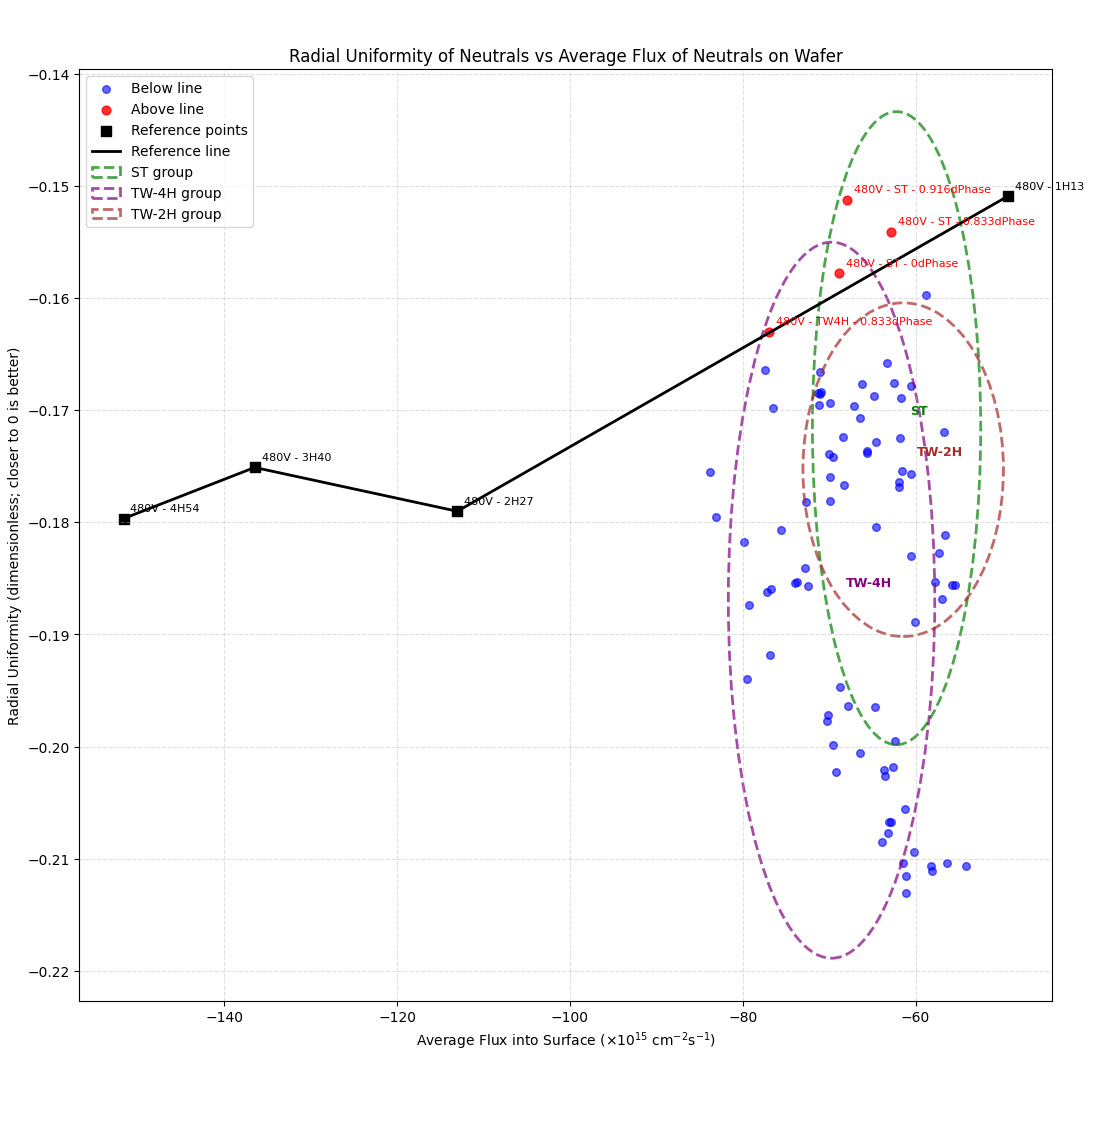
\includegraphics[width=\linewidth]{Figures/Uniformity vs Avg Flux - 0-5.2cm - Neutrals.png}
  \caption{Radial uniformity of neutrals versus average wafer flux. Several sawtooth phase settings outperform the baseline harmonic cases.}
  \label{fig:neut_u}
\end{figure}

\paragraph{Neutrals:}
 Several sawtooth phase configurations outperform the baseline in neutral uniformity at comparable (or higher) average flux, moving points closer to $U\!=\!0$. The exact mechanism for control of the neutral flux via alteration of applied fields (via TVW (Tailored Voltage Waveforms)) was not determined in this study. It is useful to not that the regions of highest neutral flux, shown previously in figure 3, correspond to the wafer and ICP dielectric surfaces - i.e. where the highest voltage sheaths would be. It is reasonable to assume that the neutral momentum in these regions is dictated by the local ion-neutral charge exchange collisions, where ions lose a charge and join the neutral species while maintaining their momentum. It is likely therefore that control of the neutral flux is mediated by first altering the sheath-localised ion dynamics, which indirectly alters the neutral dynamics via ion-neutral charge exchange. If true, the degree of control would be highly temperature and pressure dependant, however this was not addressed in this study. Interestingly the general shape of our configurations seem to be retained albeit more spread out for neutrals than positive ions.


\begin{figure}[H]
  \centering
  % \includegraphics[width=0.82\linewidth]{Uniformity_vs_Avg_Flux_-_0-5.2cm_-_Positive_Ions.png}
  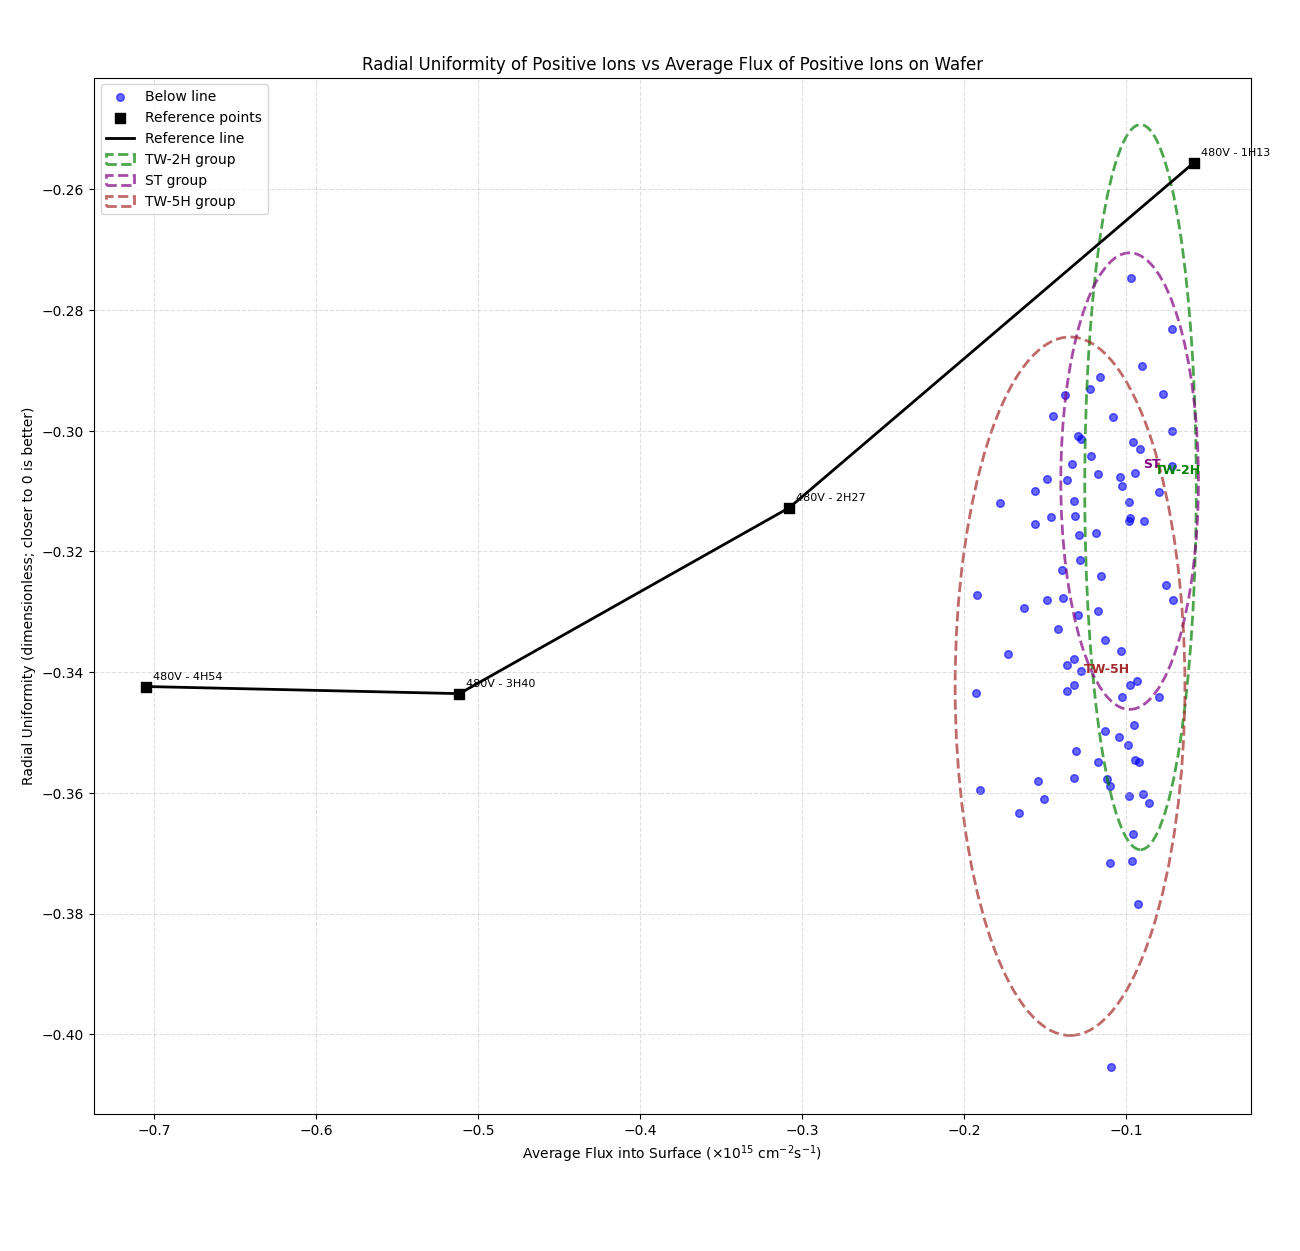
\includegraphics[width=\linewidth]{Figures/Uniformity vs Avg Flux - 0-5.2cm - Positive Ions.png}
  \caption{Radial uniformity of positive ions versus average wafer flux. No general improvement over the baseline harmonic envelope is observed.}
  \label{fig:ion_u}
\end{figure}

\paragraph{Positive ions:}
In contrast, across all tailored-waveform cases we do \emph{not} observe a systematic improvement over the baseline harmonic cases at fixed average flux; tailored points tend to sit on, or slightly above, the baseline trend. We speculate that the lack of control observed in the ions is due to the geometry, where sheath expansion and collapse heating at the edge of the wafer creates a localised increase in plasma and ion densities. The geometry does not include a focus ring which can be used to help control the sheath of the plasma, however in the GEC geometry it is not present. However we can see that the wafer surface DC self bias is being moderated due to the accurate control of power shown in Figures \ref{fig:pf_bias} and \ref{fig:st_bias}

\paragraph{Overall:}
From figures 5 and 6, we can clearly see a large variation in the uniformity (Neutral: ~33.3\%, Ion: ~35.3\%) whilst having confined control over the flux space, essentially allowing the selection of a variety of uniformity values given an average flux value. 



\subsection{RF-bias control via phase}
Figures~\ref{fig:pf_bias} and \ref{fig:st_bias} show the RF bias at $r=4.6$cm versus phase for 'peak and fall' and 'sawtooth' waveforms. Varying the phase (and the amount of harmonics) shifts the cycle-average wafer bias. In practice, this provides a handle to counteract the RF-induced self-bias: by selecting a phase that drives the time-averaged RF bias toward zero, the ion energy control reduces to the applied DC bias alone. This decoupling is desirable for independently tuning flux (via plasma sustainment) and energy (via DC bias), though complete cancellation will remain geometry and operating-point dependent.

\begin{figure}[H]
  \centering
  % \includegraphics[width=0.9\linewidth]{Peak_and_Fall_-_Harmonics_Potential_vs_Phase.png}
  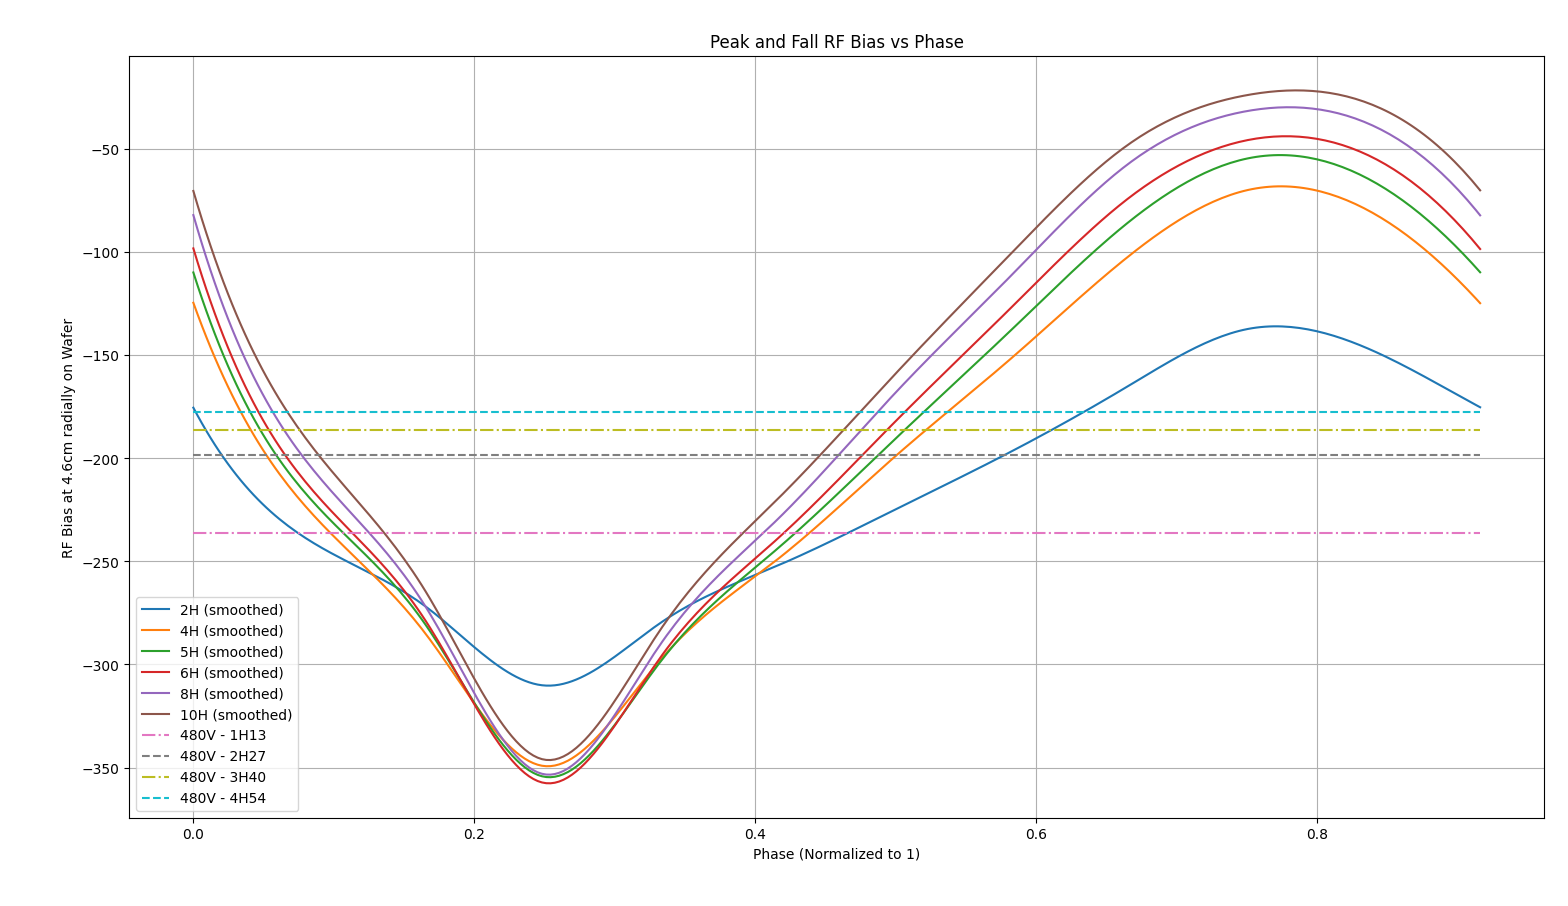
\includegraphics[width=\linewidth]{Figures/Peak and Fall - Harmonics Potential vs Phase.png}
  \caption{Peak and Fall waveform: RF bias at the wafer versus phase for multiple harmonic counts.}
  \label{fig:pf_bias}
\end{figure}

\paragraph{Peak and Fall:}
For the peak-and-fall waveform (Fig.~\ref{fig:pf_bias}), the self-bias voltage exhibits a strong dependence on harmonic phase, with the most negative bias occurring between 0.25–0.35 of the normalized phase. Increasing harmonic content systematically increases the tunability window, allowing bias control of nearly 200 V relative to the sinusoidal baseline. This highlights the potential of harmonic tailoring to decouple ion energy control from plasma density sustainment.

\begin{figure}[H]
  \centering
  % \includegraphics[width=0.75\linewidth]{Sawtooth.png}
  \includegraphics[width=\linewidth]{Figures/Sawtooth.png}
  \caption{Sawtooth waveform: RF bias at the wafer versus phase.}
  \label{fig:st_bias}
\end{figure}

\paragraph{Sawtooth:}
For the sawtooth waveform (Fig.~\ref{fig:st_bias}), phase variation similarly alters the wafer bias, but the overall control range is more modest (~100–150 V). The dependence is more sinusoidal in form, lacking the sharper bias extremes seen in peak-and-fall. Thus, while sawtooth waveforms modulate the DC self-bias voltage to a smaller degree, the 'wider' minima and maxima provide more margin for error in an operational system, which may provide more utility in practice.

\section{Conclusion}
\label{sec:conclusion}

We investigated the impact of tailored voltage waveforms on radial flux uniformity at the wafer in SF$_6$ plasmas using the HPEM at the fixed operating parameters considered (480~V peak, 10~mTorr,GEC geometry).

Control of the uniformity of neutral and positively charged fluorine onto a dielectric wafer was demonstrated with the application of tailored voltage waveforms. Neutral uniformity was improved above the single frequency baseline for cases employing sawtooth waveforms, while no cases exhibited improved uniformity for positive ion species. This lack of improvement is attributed primarily to the GEC geometry, most notably additional ionisation mechanisms present at the radial extrema of the wafer. This work illustrates that careful consideration of the geometry is required when applying electromagnetic control systems.

It can be seen that the control on the time averaged RF bias can be significantly altered by the use of tailored waveforms, specifically for the peak and fall waveform in which we can see a 50\% down-medulation and a over 90\% up-modulation.

Further work could look at applying these configurations to actual OIPT geometry where the electrode is on the top of the reactor rather than near the wafer. It would also be of interest to be able to nullify a self bias using tailored waveforms. A nullifying the self bias makes it much easier to control the ion energy. Further work could also investigate thoroughly into the ion energy distribution using the HPEM.

Overall, tailored waveforms offer a practical handle for improving neutral flux uniformity in GEC geometry and for managing wafer bias in SF$_6$ plasmas. Realising comparable gains for ions will likely require combining waveform control with modest geometric or operating-point changes.



\addcontentsline{toc}{section}{Bibliography}

\newpage
\printbibliography
%~~~~~~~~~~~~~~~~~~~~~~~~~~~~~~~~~~~~~~~~~~~~~~~~~~~~~~~~~~~~~~~~~~~~~~~~~~~~~~~~~~~~~~~~~~~~~~~
%~~~~~~~~~~~~~~~~~~~~~~~~~~~~~~~~~~~~~~~~~~~~~~~~~~~~~~~~~~~~~~~~~~~~~~~~~~~~~~~~~~~~~~~~~~~~~~~
%~~~~~~~~~~~~~~~~~~~~~~~~~~~~~~~~~~~~~~~~~~~~~~~~~~~~~~~~~~~~~~~~~~~~~~~~~~~~~~~~~~~~~~~~~~~~~~~
\end{document}
 


%Fin :) - Happy Typesetting!